\chapter{Problem Statement \& Proposed Solution} \label{chap:proposed-solution}

\section{Problem Statement}

\begin{comment}
	* Mention smart grids iin the end of scope?
\end{comment}

As addressed in the previous chapter, graphs are ubitquotous representations that can serve to instinctively represent several problems and domains. In some problems these representations reveal underlying features that can't be naturally represented by plain euclidean data. However, this problem becomes even more complex considering that graph data is complex and there is a need for designing methods that efficiently extract representations. \par
By conduction a thorough literature review of the relevant studies in the field we observed that current \ac{RL} algorithms are not prepared to handle such complexity by considerind envrionment graph topology features in the decision making process, which deeply affects the performance of decision-making systems inserted in graph-based domains. Additionally, they lack an efficient method for generalizing the learned policies in dynamic topologies that suffer changes over time.
 \par
This problem can be observed in several studies where RL models are applied to domains where the intricate relationships between the objects may be relevant for mapping the observable environment states to optimal action policies. Smart Grid services are an example of such domains, given that power grids can be viewed as complex networks of nodes (consumers or producers) and powerlines connecting them that transport energy. 
More and more, this issue attracts the curiosity of academics. With the recent advancements of GNNs the popularity around \ac{GRL} has rose because of their excellent efficiency in creating optimal graph representations and other graph machine learning problems.

\subsection{Scope}

This dissertation will focus on studying this problem in the context of single-agent \ac{RL} algorithms, given that multi-agent systems are significantly more complex to implement. Furthermore, in the context of the disseration's application domain, which is smart grid services, the possible improvements in \ac{GRL} techniques will be implemented to the \acf{DED} problem that studies solutions that optimze power generation cost while maintaining reliable grid stability. Additionally, the \ac{GRL} proposed models may be also implemented to solve other smart grid systems such as Undervoltage Load Shedding and Volt-VAR Regulation.

\section{Requirements}

\subsection{Functional}

\begin{table}[h!]
	\centering
	\caption{Functional Requirements}
	\begin{tabular}{|P{1cm}|P{3cm}|p{10cm}|  }
		\hline
		\textbf{FR} & \textbf{Title} & \textbf{Description} \\
		\hline
		F1 & Optimization & The system should be able to optimize the dispatch of generation resources in real-time by managing generator power levels to meet the time-varying load demands \\
		\hline
		F2 & Graph Features Extraction & The system must implement a grah machine learning mechanism for creating and generalising efficient representations of the environment \\
		\hline
		F3 & Learning Capability & The system must learn from past experiences and optimize its dispatch policies over time \\
		\hline
		F4 & Adaptability & The system should adapt to changes in the power grid topology or in load patterns \\
		\hline
		F5 & Constraints & The system should fullfil the various power grid constraints, namely power balance, generator constraints, ramp rate limits and \ac{ESS} Constraints \\
		\hline
		F6 & Scalability & The system must handle scenarios of different sizes, ranging from small to complex power distribution grids \\
		\hline
		F7 & Monitorization & The system must implement tracking mechanisms in order to gather the different metrics, namely: 
		\begin{itemize}
			\item Convergence Rate
			\item Training Time
			\item Computation Time
			\item CPU/GPU Utilization
			\item Operating Cost
		\end{itemize} 
		in order to enable the comparative and evaluative process between the different models. \\
		\hline
	\end{tabular}
\end{table}

\subsection{Non-functional}

\begin{table}[h!]
	\centering
	\caption{Non-functional Requirements}
	\begin{tabular}{|P{2cm}|P{4cm}|p{6cm}|  }
		\hline
		\textbf{Requirement} & \textbf{Title} & \textbf{Description} \\
		\hline
		NF1 & Performance & \\
		\hline
		NF2 & Reliability & \\
		\hline
		NF3 & Usability & \\
		\hline
		NF4 & Security & \\
		\hline
		NF5 & Maintainability & \\
		\hline
		
		\hline
	\end{tabular}
\end{table}

\subsection{Structural}

\section{Architecture} \label{sec:arch}

\begin{comment}
	* Mathematical Formulation of Actions vs States
\end{comment}

Considering the conclusions taken from the reviewed literature, in chapter \ref{chap:literature-review}, our proposed solution combines efficient \acf{DRL} approaches with \acfp{GNN}, the state-of-the-art approach for graph representation learning. Generally, the system receives graph-based representations of the environment and encodes them using the \ac{GNN} algorithm. By also leveraging deep learning techniques, \ac{DRL} maps the encoded embeddings to optimal action sequences with the goal of meeting the real-time load demand and reducing the operating cost of the power distribution grid. The general architecture of the solution can be observed in figure \ref{fig:arch}.

\begin{figure}
	\centering
	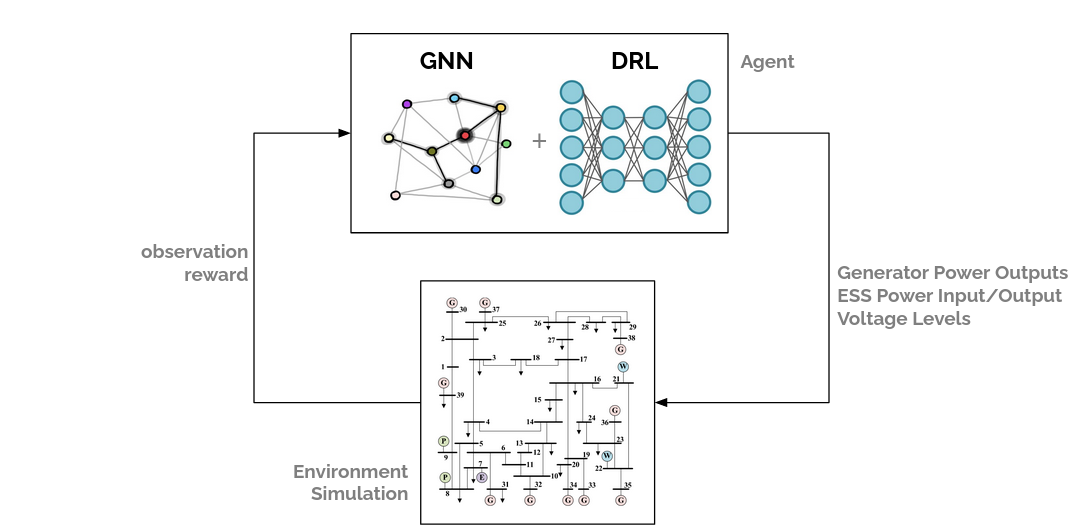
\includegraphics[width=0.85\linewidth]{./figures/arch.png}
	\caption{Solution Architecture}
	\label{fig:arch}
\end{figure}


To fullfil this, the agent adjusts the generator power output and voltage levels and manages the \ac{ESS} operation in real-time. \par
The solution is executed in the context of a power grid simulation that models the approapriate elements, properties, constraints and operating of the power distribution grid. This method is further described in the upcoming subsection \ref{sec:method}.

\section{Methodology} \label{sec:method}

\begin{comment}
	* Constraints 
	* Element Attributes 
	* Python
	* PyTorch, PyG for GNNs?
	* Evaluative mehtods as subsection?
	* GIT Repo?
\end{comment}

Regarding the established methodology for enabling the implementation of the proposed solution, the Grid2Op framework \cite{rtefranceGrid2OpDocumentation}  will be used for modeling the sequential decision-making process on simulated power distribution grid. Grid2Op is designed by RTE (Réseau de Transport d'Électricité), the electricity transmission system operator of France, and is equipped with a variety of pre-defined scenarios used in coding competitions and based on real-world data. This platform focuses on easing the job using the grid topolgy to control the power flows and also allowing for it to be reconfigured in real-time. Additionally, enables to graphically plot the current observable state of the grid, as portrayed in figure \ref{fig:grid2op-graph}. Apart from graph topology, grid2op also enables the manipulation of:

\begin{itemize}
\item the \textbf{voltages} by manipulating the setpoint value of the generators;
\item the \textbf{active generation} by using the 
\end{itemize}

This framework is compatible with the Gymnasium framework \cite{faramafoundationGymnasiumDocumentation}, a widely used toolkit for developing \ac{RL} algortihms, which will also be used in this work together with the Grid2Op simulation environment. 

\begin{figure}
	\centering
	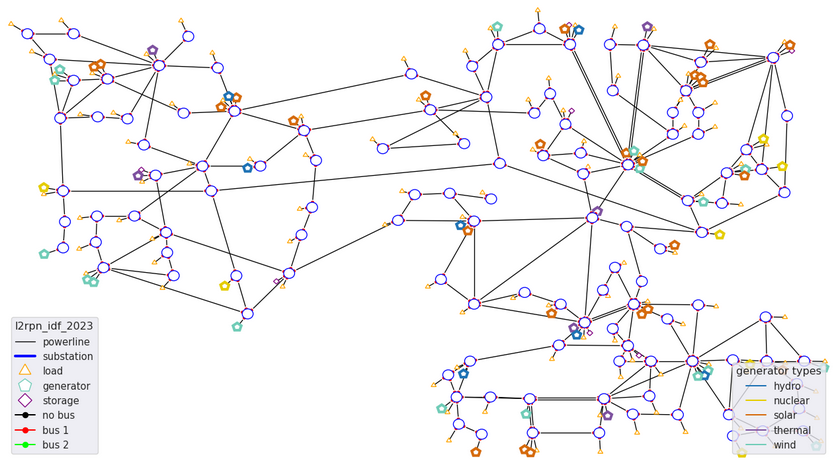
\includegraphics[width=0.85\linewidth]{./figures/grid2op-graph.png}
	\caption{Grid2Op l2rpn\_idf\_2023 scenario \cite{rtefranceGrid2OpDocumentation}}
	\label{fig:grid2op-graph}
\end{figure}

This platform focuses on describing the power distribution grids by modeling the following objects:
\begin{itemize}
	\item \textbf{Buses} are the fundamental objects of the power grid, representing nodes where power sources, loads and other elements are connected.
	
	\item \textbf{Powerlines} represent edges in the power grid and connect the different buses together. They represent the physical transmission and distribution lines and allow power to flow from one part of the grid to another
	
	\item \textbf{Generators} are critical grid elements connected to buses whose main role is to produce power and maintain grid stability by balancing the energy supply and demand. They can be Conventional Thermal Generators, Wind Turbines or Photovoltaic Cells.
	
	\item \textbf{Loads} consume power from the grid, simulating electricity use. They're also associated to an individual bus.
	
	\item \textbf{Storage Units} can act as both consumers and producers. They're able to retain energy from the power grid when producion surpasses demand for later injecting bacck power when convenient. Storage units are bound by a maximum energy storage capacity.
\end{itemize}


The different combinations of algorithms will be applied to a set of modified scenarios that fulfill the settled requirements. For Deep Reinforcement Learning algortithms, solutions with plain \ac{SAC}, \ac{DDPG} and \ac{PPO} approaches and combined with the \ac{GCN}, \ac{GAT} and \ac{GIN} architectures. Concerning result analysis, it's also important to point out the use of quantitative methods for evaluating the different implemented models, a topic that is further explored in the following section \ref{sec:eval-methods}.


\section{Evaluative Methods} \label{sec:eval-methods}

\begin{comment}
	* Sample Efficiency
	* Other methods
\end{comment}

The solution described in the previous subsections \ref{arch} and \ref{sec:method} clearly involves intricate operational mechanisms, something that calls for a sophisticated evaluative process. Furthermore, given the comparative nature of this disseration the evaluation and analysis methods will be key factors in studying and confronting the different combinations of \acp{GNN} and \ac{DRL}, as well as possible improvements in the integration of these techniques.
In this manner, we define the four dimensions for evaluating and analyzing the different \ac{GRL} models:

\begin{description}
	\item[Learning efficiency] This dimension assesses how effectively the models learn and improve their decision-making process over time. It involves evaluating how quickly they converge to optimal or near-optimal dispatch strategies through the convergence rate. 
	
	\item[Computational Efficiency] It's crucial that the solution is able to perform well on real-time execution. In this context, not only it's important to assess the solution's decision computation performance but also to measure the time necessary for the model offline training, as well as the observed CPU/GPU resource utilization.
	
	\item[Dispatch Efficiency] The performance of the \ac{GRL} model in managing power distribution from the various generators will be mainly measured by the daily operating cost (in \textit{Euros}) derived from the agent's sequence. Furthermore, other system behaviors will be analyzed such as Renewable Energy Source Penetration and Energy Storage System utilization.
	
	\item[Scalability and Adaptation]  The solution will be applied to scenarios of several sizes for analyzing its scalability. Furthermore, we will induce variations in the simulation scenarios to test the model's ability to handle toplogy changes.
\end{description}

\section{Work Plan}

In order to make this project possible, we propose a 40-week work plan divided into four stages, whose start was in the last week of september 2023 and expected conclusion is scheduled for the last week of June 2024, observable in figure \ref{fig:gantt-chart}. \par
The first stage, ranging from the first week of the plan to the delivery of this report, encompasses the \textbf{disseration preparation} phase. This stage mainly addressed the initial knowledge acquisition necessary to understand this work's context and gather a basic grasp on the concepts and topics it addresses, namely:
\begin{itemize}
	 \item Reinforcement Learning
	\item Graph Theory
	\item Graph Representation Learning
	\item Graph Reinforcement Learning
	\item Graph Neural Networks
	\item Smart Grids Services
\end{itemize}
This process is followed by the analysis of existing research and approaches in \ac{GRL} and Smart Grid technologies which spans till the first week of January 2024, documented in chapter \ref{chap:literature-review}. Lastly, the preparation phase is also compromised of the PDIS report write-up until its delivery in the first week of Ferbruary 2024, marking the end of this phase. \par
The preparation phase is followed by the \textbf{Development} phase. This stage encompasses all activities related to the system implementation, from the preparation of the simulation environment to the model training and calibration. The development phase spans from the first week of February 2024 to the second-to-last week of April 2024. \par
Next, the \textbf{Evaluation \& Analysis} stage is set, compromising the time frame where the various implemented models will be evaluated in the context of the previously mentioned dimensions and the evaluation results will be analyzed. \par
Lastly, the \textbf{Disseration} write-up and subsequent revision work will be performed, compromised of the write-up, proofreading and correction tasks and ranging from the end of the evaluation and analysis phase in the last week of April 2024 until the last week of the plan.

\begin{figure}
	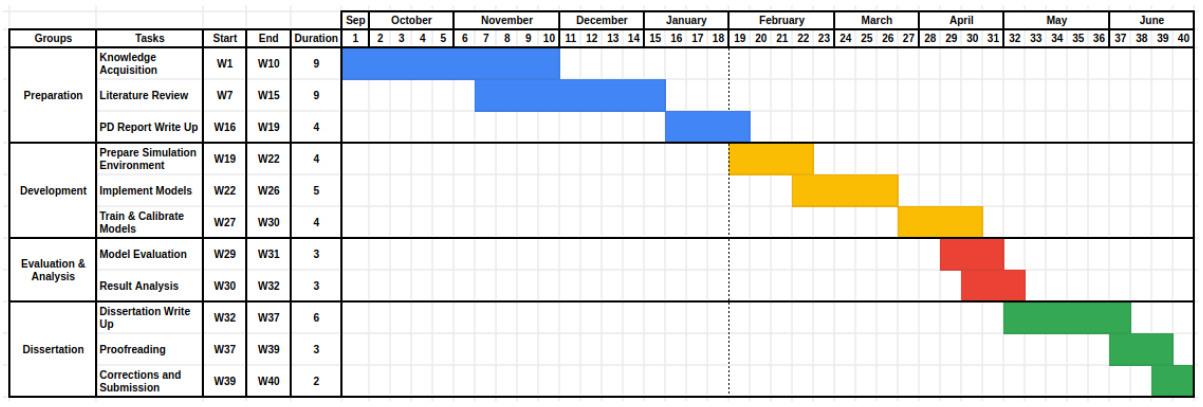
\includegraphics[width=1.0\linewidth]{./figures/gantt-chart.png}
	\caption{Dissertation Work Plan Gantt Chart}
	\label{fig:gantt-chart}
\end{figure}

